\begin{frame}
	\frametitle{Процес створення маски рухомих об'єктів алгоритмом Б-К}
	\begin{figure}[H]
		\centering
		\subfloat[Попередній кадр $F^i$]{
			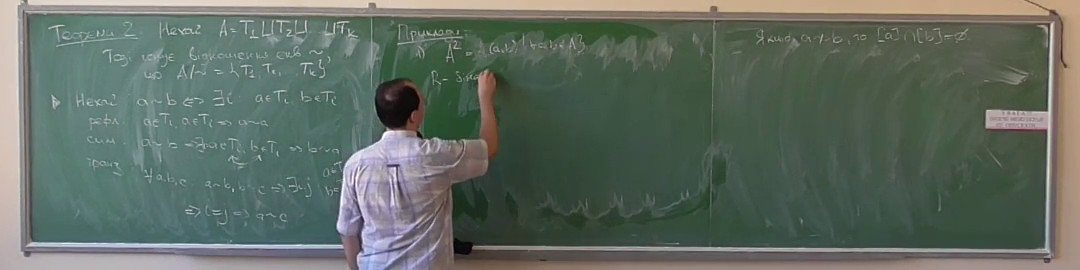
\includegraphics[width=0.45\textwidth]{images/prev_frame}
		} \quad
		\subfloat[Поточний кадр $F^{i+s}$]{
			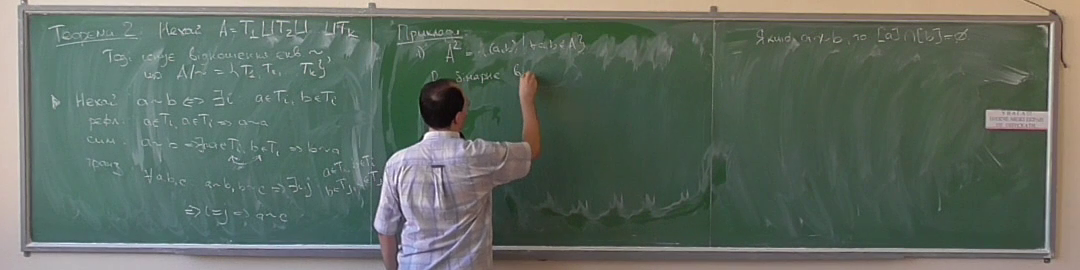
\includegraphics[width=0.45\textwidth]{images/next_frame}
		}\\
		\subfloat[Інвертована різниця $F^i$ і $F^{i+s}$]{
			
\includegraphics[width=0.45\textwidth]{images/inv_diff}
		} \quad
		\subfloat[Маска рухомих об'єктів на кадрі $F^{i+s}$]{
			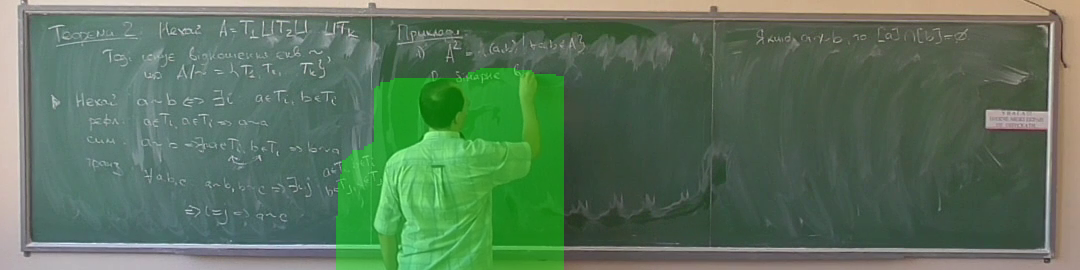
\includegraphics[width=0.45\textwidth]{images/next_with_mask}
		}
		\caption{Джерело ~---~ \url{https://youtu.be/a7TUp4p-pIk}
		}
	\end{figure}
\end{frame}
